%----------------------------------------------------------------------------
\chapter{\bevezetes}
%----------------------------------------------------------------------------

Egy monitor feladata az, hogy futási időben egy rendszert megfigyeljen, elemezzen és egy adott követelmény alapján felismerje a rendszer helytelen viselkedését. Ezt a helytelen viselkedést jelzi a rendszernek, de néhány esetben a rendszer működését is befolyásolhatja. Egy rendszer viselkedése lehet kontextusfüggő, amit a monitornak figyelembe kell venni. Például, egy gépjármű fékezésének vezérlését befolyásolja a terep, amin épp halad. A rendszer működése tehát függ a környezetétől. Ezért, hogy a viselkedését ellenőrizni tudjuk, a monitornak információval kell rendelkeznie a környezetben történő változásokról. Ezen kívül, a monitornak időmérésre is szüksége van, mert a követelmény tartalmazhat időziteseket is. Az 1. ábra bemutatja a monitorozás koncepcióját.

\begin{figure}[!ht]
    \centering
    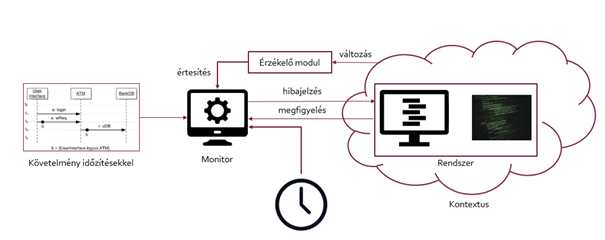
\includegraphics[width=150mm, keepaspectratio]{figures/1abra.png}
    \caption{Kontextusfüggő rendszerek monitorozása időzítési feltételekkel.}
\end{figure}

A scenario alapú monitorozás során a kommunikáció megfigyelésével szeretnénk felismerni a problémákat a rendszerünkben. A rendszerben lévő objektumok közti interakciókat, üzeneteket fogja megfigyelni a monitor. A követelményt scenario formájában adjuk meg az üzenet szekvenciák specifikálására. Szekvencia diagramok segítségével egyszerűen megadhatunk ilyeneket. A diagramokat a későbbiekben olyan alakra kell majd hoznunk, hogy abból a monitor létrehozható legyen.
